\documentclass[a4paper, twoside, 11pt]{article}
\usepackage[margin=1.5cm]{geometry}
\usepackage[]{xcolor}
\usepackage{cite}
\usepackage{graphicx}
\usepackage{listings}
\usepackage{float}
\usepackage{amsmath}

\lstset{frame=tb,
  language=Java,
  aboveskip=3mm,
  belowskip=3mm,
  showstringspaces=false,
  columns=flexible,
  basicstyle={\small\ttfamily},
  numbers=none,
  numberstyle=\tiny\color{gray},
  keywordstyle=\color{blue},
  commentstyle=\color{dkgreen},
  stringstyle=\color{mauve},
  breaklines=true,
  breakatwhitespace=true,
  tabsize=3
}

\definecolor{dkgreen}{rgb}{0,0.6,0}
\definecolor{gray}{rgb}{0.5,0.5,0.5}
\definecolor{mauve}{rgb}{0.58,0,0.82}

% define the title
\author{L. ~Towell, L.M.Towell@liverpool.ac.uk}

%defines the title
\title{Assignment 1\break Brute Force Attack Estimation}

\begin{document}
	%generate the title
	\maketitle

\maketitle
\section{Password List}
Below is the password list that I have decided to use for this exercise.
\begin{center}
	\begin{tabular}{ |c|c| } 
	 \hline
	 N & Password \\
	 \hline
	 1 & abc \\ 
	 2 & P@ssW0rD \\ 
	 3 & Th!\$IsAV3ryL0n9pA\$\$w0rd \\ 
	 \hline
	\end{tabular}
\end{center}

\section{Salt and Iteration Count}
For the purpose of this coursework I have hardcoded the salt used within this program, 
I have also decided to use an iteration count of 1024. The below table shows the time per run and the average time
 taken in milliseconds over 5 iterations to encrypt and decrypt the string "This is an example string" using the 
 defined salt and iteration counts.

 The below timings have been recorded running the program on a Macbook air with an Intel core i5 processor and 16GB of RAM.
  Timings on other machines are likely to differ.
 \begin{center}
	\begin{tabular}{ |c|c|c|c| } 
	 \hline
	 \multicolumn{4}{|c|}{Iteration time in milliseconds (ms)} \\
	 \hline
	 N & abc & P@ssW0rD & Th!\$IsAV3ryL0n9pA\$\$w0rd \\
	 \hline
	 1 & 155.77 & 2.45 & 1.46 \\ 
	 2 & 8.55 & 1.66 & 1.19  \\ 
	 3 & 6.27 & 1.65 & 1.24  \\ 
	 4 & 12.94 & 4.0 & 1.25 \\
	 5 & 1.57 & 2.01 & 2.69  \\
	 \hline
	 \hline
	 Average & 7.33 & 2.35 & 1.57  \\
	 \hline
	 \multicolumn{4}{|c|}{The first iteration of abc has been omitted from the average} \\
	 \hline
	\end{tabular}
\end{center}

\section{Brute Force Attack Estimation}
Given that it is specified that the attacker knows the salt, iteration count, encryption type, 
input string and cipher text used to encrypt the input string then the only piece of information 
the attacker would need to find is the password used to encrypt the string. 
In order to work out the password using a Brute force attach the attacker is going to have to 
iterate through each possible character that could be used in each different combination.

If we presume that passwords are made of uppercase, lowercase numbers and special characters and they are
limited to traditional ASCII encoded characters then this gives the attacker a possible 95 characters for each character in the password.
The equation for working out a password via brute force attack is therefore $95^n$ where n is the number of characters within the password.
The table below shows the amount of possible combinations for N character lengths.

\begin{center}
	\begin{tabular}{ |c|r| } 
	 \hline
	 Number of characters & Possible password combinations \\
	 \hline
	 1 & 95 \\
	 2 & 9025 \\
	 3 & 857375 \\
	 4 & 81450625 \\
	 5 & 7737809375 \\
	 6 & 735091890625 \\
	 7 & 69833729609375 \\
	 8 & 6634204312890620 \\
	 9 & 630249409724609000 \\
	 10 & 59873693923837900000 \\
	 15 & 463291230159753000000000000000 \\
	 20 & 3584859224085420000000000000000000000000 \\
	 23 & 3073568677250240000000000000000000000000000000 \\
	 25 & 27738957312183400000000000000000000000000000000000  \\
	 \hline
	\end{tabular}
\end{center}

In order to estimate the time taken to brute force an attack we need to look at the time taken to iterate through every combination possible
 considering that in the worse case the last combination will be the password we are attempting to discover.
The calculation for estimating time taken to discover a password is therefore the time taken to try one password (one iteration)
 mutliplied by the number of possible combinations. For example if we say the time taken for 1 iteration is 1ms then we can assume that it
 would take in the worst case to crack a 3 character password (abc) which would be $95^3$ (857375 combinations) * the taken to complete one
 iteration e.g. 1ms per attempt would take 857375ms or 857.375 seconds or 14.3 minutes.

 \textit{Figure. 1} is a table of estimated time taken to discover passwords of varying character lengths using the brute force method. 
 You can see that the longer the character length the longer the time taken growing to time periods which will never be broken within
  our lifetime after just 5 characters. 

  Taking \textit{Figure. 1} into account I have estimated the time taken to break my passwords using my average encryption time of 1.56ms per iteration in the table below.

  \begin{center}
	\begin{tabular}{ |l|c|r| } 
	 \hline
	 Password & characterLength & Estimation to discover \\
	 \hline
	 abc & 3 & 142.5ms \\
	 P@ssW0rD & 8 & 315,554 years \\
	 Th!\$IsAV3ryL0n9pA\$\$w0rd & 23 & 105 Septillion Years \\
	 \hline
	\end{tabular}
\end{center}

  \newpage

\begin{figure}[H]
	\centering
	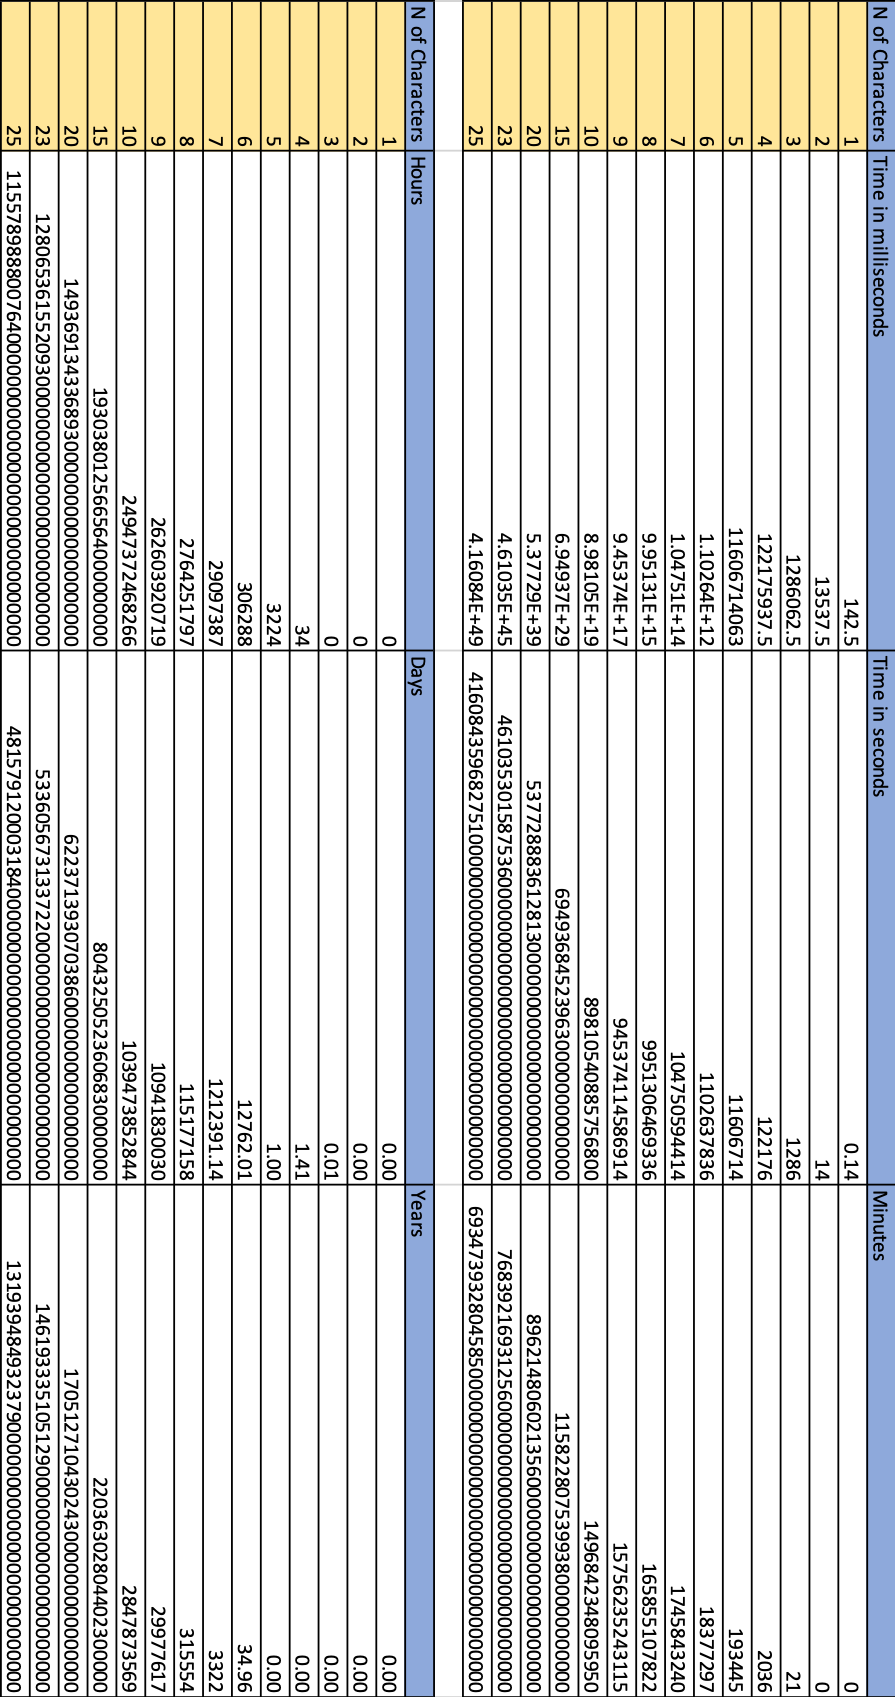
\includegraphics[scale=0.9]{Images/timeEstimationImage.png}
	\caption{Table of time taken to discover characters assuming 1 iteration takes 1 millisecond.}
\end{figure}

\section{How Does Iteration Count Affect Brute Force Timing?}
What does iteration count mean?

What is the maximum value of iteration count?

\section{Brute Force Attack Estimation Without Known Iteration Count}
Essentially if a hacker does not know the iteration count of an application then they have to try the same brute
force attack multiple times for multiple iteration counts which essentially means that the time taken grows exponentially.
E.g. If the iteration count was 300 and the hacker started their hack attempt with an iteration count of 1 they would have
to work out the characters in the password $95^n*i$ where $i$ is the number of iterations needed to reach the one initially
used when hashing the password.



\section{Comparison with Online Services}
\begin{center}
	\begin{tabular}{ |c|c|c| } 
	 \hline
	 Password & My Estimation & Online Estimation  \\
	 \hline
	 abc & 400 ns & 1 \\ 
	 P@ssW0rD & ? & 9 hrs \\ 
	 Th!\$IsAV3ryL0n9pA\$\$w0rd & 1 & 19 Septillion Years \\ 
	 \hline
	\end{tabular}
\end{center}

\newpage
\section*{Appendices}
\appendix
\section{Password Encryption \& Decryption Program}
\lstinputlisting{../code/PasswordBasedEncryption.java}
\newpage
\section{Output of Appendix A when ran in terminal}
\lstinputlisting{../code/timings.txt}

\end{document}